\section{Introdução}\label{sec-introdução}

Em Moçambique, ainda há grandes desafios na adoção efetiva das
Tecnologias Digitais de Informação e Comunicação (TDICs) nas salas de
aula. Especificamente, o ensino de disciplinas como Desenho Técnico (DT)
e Geometria Descritiva (GD) permanece ancorado em métodos tradicionais,
utilizando apenas recursos convencionais, como quadro negro, giz, réguas
de madeira/plástico, lápis e borracha. É evidente a escassez de Recursos
Tecnológicos (RTs), como computadores, projetores, tablets e
smartphones. O acesso limitado à internet e aos computadores representa
uma das principais barreiras ao progresso educacional em Moçambique. \textcite[p. 16]{ali2018} argumentam que, em Moçambique, as relações
computador/utilizador \enquote{são os principais desafios identificados no
domínio das Infraestruturas} escolares. É importante observar que, no
contexto educacional moçambicano, o uso de tecnologia frequentemente se
restringe aos conteúdos de TDICs, como os pacotes básicos da Microsoft
Office, à plataforma Moodle (utilizada para o Ensino a Distância no
Ensino Superior) e a alguns programas de televisão que abordam temas do
Ensino Secundário Geral (ESG).

Os alunos demonstram menor interesse nas disciplinas que abrangem
conteúdos de DT. Na opinião deles, os temas são de difícil compreensão,
devido à abstração relacionada à Visualização Espacial (VE) 3D e à sua
representação no plano bidimensional (folha de desenho). Por um lado, os
alunos enfrentaram dificuldades na VE 3D, e, por outro lado, ESG público
é tradicionalmente ministrado sem o uso de qualquer RT. O regulamento
interno do ESG proíbe o uso de smartphones como meio didático para
aprendizagem em sala de aula. Esses dispositivos portáteis acessíveis
poderiam substituir os computadores, já que permitem uma representação
dinâmica em 3D dos elementos geométricos. Com o avanço da tecnologia,
foram desenvolvidos softwares suportados em smartphones, nos quais os
elementos geométricos são modelados, possibilitando a comparação com a
representação dos mesmos elementos em Aplicativos Tecnológicos (ATs) no
plano bidimensional da folha de desenho em 2D.

Nesse contexto, o ensino em Moçambique é tradicional, ministrado sem o
auxílio de RTs que facilitam a representação em 3D, o que pode
contribuir para a dificuldade dos alunos do ESG na VE em 3D; por isso,
optou-se por selecionar dois ATs para a presente pesquisa: o Qubism 3D
Modeling (Q3DM) e o software de geometria dinâmica GeoGebra. Ambos os
aplicativos têm potencial para promover a VE. Daí surge a pergunta de
pesquisa: De que modo os aplicativos Qubism 3D Modeling e software de
geometria dinâmica GeoGebra, adaptado para smartphone, melhora a
visualização espacial no estudo das Projeções Ortogonais (POs) e Secções
de Cilindros (SCs)?

A tecnologia oferece uma vantagem significativa para a nova geração de
nativos digitais, que cresceram imersos em um ambiente tecnológico. Eles
têm uma habilidade natural para aprender utilizando ATs, o que facilita
a compreensão de conteúdos complexos de diversas disciplinas. Segundo
\textcite[p. 1]{prensky2001}, ao se referir a esses alunos como \enquote{Nativos
Digitais}, ele destaca que eles são fluentes na linguagem digital dos
computadores, videogames e internet. Essa familiaridade com a tecnologia
faz com que os alunos atuais tenham facilidade no uso de ATs,
influenciando positivamente sua conexão com os conteúdos educacionais.
Por outro lado, grande parte dos professores, que podem ser considerados
emigrantes digitais, enfrentam o desafio de ensinar aos nativos digitais
com o auxílio da tecnologia. Para isso, os professores precisam se
adaptar aos recursos tecnológicos e à sua linguagem, a fim de facilitar
a aprendizagem dos alunos na sala de aula. As tecnologias oferecem um
suporte eficiente para a elaboração de projetos inovadores e de
qualidade.

\subsection{Tecnologia na educação}\label{sub-sec-tecnaeducação}
As tecnologias adequadas à educação podem ser utilizadas como
ferramentas pedagógicas para auxiliar o processo de ensino e
aprendizagem de forma colaborativa e interativa. Tais tecnologias
promovem efetivamente novas formas de ensinar e aprender,
potencializando o desenvolvimento de novas competências \cite[p. 83]{baeta2018}. Para os autores, as tecnologias na educação têm
importância na formação dos alunos, pois podem despertar o interesse
deles, impulsionando o desenvolvimento de novas competências.

Especificamente nas disciplinas de DT e GD, a tecnologia surge pela
necessidade de representar em 3D todos os elementos geométricos e sua
dinâmica no espaço, promovendo a capacidade de visualizar em 3D e a
percepção da dinâmica dos elementos geométricos no espaço. Tais
tecnologias fornecem informações que possibilitam a construção do
conhecimento abstrato, auxiliando na melhoria da aprendizagem dos alunos
e na mediação do professor. Por isso, \textcite[p. 1122]{novoa2017} defende que
\enquote{[$\ldots$] um professor deve se preparar para agir num ambiente de
	incerteza e imprevisibilidade} \textcite[p. 3]{brito2010}; “no mesmo pensamento,
defende que por isso, deverá estar atenta às inovações tecnológicas para
benefício do sucesso educativor”. Os autores supracitados sugerem que o
professor, hoje, deve aprender e adaptar-se às novas tecnologias,
utilizando-as como ferramentas a seu favor, para facilitar em qualquer
modelo de ensino e em todos os conteúdos teóricos. É notável a
facilidade com que os alunos se motivam, quando interagem com a
aprendizagem, auxiliados pelos ATs. O professor, além do poder de
selecionar a tecnologia adequada para a sua aula, também se beneficia da
eficiência para esclarecer os conteúdos. Assim, o uso da tecnologia na
Educação pode garantir uma mediação interativa no processo de ensino e
aprendizagem.

Sua implementação-educação trouxe uma nova forma de ensinar e de
aprender, transformando conteúdos complexos em simples. Nessa
tranformação-informação chega ao aluno de forma dinâmica e interativa.
Sua progressão impactou em novos métodos e meios de ensino/aprendizagem,
especialmente em aplicativos instalados em computadores, \textit{tablets},
\textit{smartphones} e na Internet \cite{siahaan2017}. Os autores mencionam
que o desenvolvimento da tecnologia possibilitou ao ensino vários
métodos de aprendizagem, e, particularmente nas disciplinas de DT e GD,
trouxeram as simulações computacionais.

É importante destacar que a sala de aula é um espaço onde o professor
pode incorporar os ATs adequados aos alunos e ao ensino. Desse modo, o
ensino não se limita à transmissão de informações, mas também é um meio
de organizar a atividade de estudo dos alunos.

\subsection{Simulações computacionais}\label{sub-sec-simulaçõescomputacionais}

A processo evolutivo da computação permitiu a prática de novos métodos
para o ensino-aprendizagem das disciplinas de GD e DT \cite{mexas2015}, por meio das simulações computacionais. Essas simulações permitem
o estudo de casos práticos através de variáveis controladas por sistema
programado; facilitam o estudo de conteúdos abstratos de forma simples e
interativa, possibilitando a análise de casos sociais ou físicos por
meio da variação de variáveis, que definem o comportamento dos sistemas.
Em tais cenários, os usuários podem participar ativamente, mesmo quando
a realidade é demasiadamente perigosa, cara, complexa, rápida ou lenta,
desenvolvendo compreensões intuitivas de fenômenos abstratos \cite{garneli2018}.

As situações imitam processos ou simulações da vida real com um modelo
limitado para manipular e examinar as relações entre variáveis
interativas de fenômenos reais, atuando como uma prática para tarefas no
mundo real \cite{kunkler2006,lamb2018}. Tais simulações têm sido
utilizadas na formação dos alunos para adquirirem competências
necessárias para executarem uma tarefa em um ambiente de baixo risco,
desenvolvendo competências de pensamento crítico e estratégico \cite{kappers2016}. Na visão dos autores, aliada ao problema da presente
pesquisa, as simulações computacionais para aprendizagem do DT e da GD
permitem que o usuário visualize os elementos geométricos em qualquer
ângulo do ponto de vista. As experiências são realizadas em um ambiente
virtual onde os sólidos geométricos são manipulados, facilitando ao
aluno praticar várias vezes o mesmo problema. As simulações
computacionais não só podem ser executadas em computadores, como também
em \textit{smartphones}, \textit{tablets} e quadros interativos. Dessa maneira, essas simulações apresentam-se como um instrumento didático potencial para a promoção do conhecimento, estimulando a aprendizagem de forma
motivadora, além de auxiliar a compreensão dos conceitos abstratos de DT
e GD.

\subsection{Aplicativos tecnológicos}\label{sub-sec-aplicativostecnologicos}

A implementação dos ATs como ferramenta didática pode trazer um leque de
alternativas para o professor mediar os conteúdos com mais facilidade,
além de estimular a curiosidade do aluno em aprender. Eles oferecem uma
qualidade significativa de ensino, visto que os alunos são incentivados
a desenvolver os pensamentos crítico e lógico, tornando-se o centro das
atenções, ao contrário do ensino tradicional, no qual o foco está no
professor. Ademais, o professor assume outras dinâmicas de ensino,
tornando-se um pesquisador digital e orientador.

As vantagens dos ATs incluem: facilidade de manipulação; possibilitam
descoberta e exploração de novas informações; permitem a construção de
elementos em 3D; estimulam a criatividade em projetos; proporcionam uma
visualização clara, facilitando comparações e análises; possibilitam
simulações computacionais nos conteúdos de DT e de GD; e garantem uma
aprendizagem significativa com qualidade. \textcite[p. 212]{silva2017}
acrescentam, argumentando que \enquote{despertam o interesse por algo que mal
	entendiam, ou acreditavam não ser tão importante conhecer, como
	conceitos geométricos tridimensionais, envolvendo o conhecimento de
	sólidos, como prismas, pirâmides, cilindros, cones e esferas}.

A abordagem da aprendizagem significativa envolve o processo pelo qual o
aluno, utilizando-se de conhecimentos e habilidades prévias, incorpora
novos conceitos. Nesse processo, o professor atua como facilitador e
interage com o aluno, proporcionando uma compreensão mais profunda dos
conteúdos abordados. Essa interação visa, principalmente, a alcançar
resultados substanciais e tangíveis no aprendizado. Esse aumento de
aprendizagem foi encontrado no estudo de \textcite{silva2017}, no qual
os autores argumentam que:

\begin{quote}
	Despertar o interesse por algo que mal entendiam, ou acreditavam não ser
	tão importante conhecer, conceitos geométricos tridimensionais,
	envolvendo o conhecimento de sólidos, como prismas, pirâmides,
	cilindros, cones e esfera. A aprendizagem significativa traz essa
	conceção, onde o aprendiz, a partir de um conhecimento e competência já
	adquiridos, agrega novos conceitos, e o professor pesquisador interage
	com o educando, contribuindo para um maior aprofundamento do conteúdo
	abordado, sobretudo, alcançando resultados expressivos \cite[p. 212]{silva2017}.
\end{quote}

Para disciplinas como DT e GD, podem ser utilizados vários aplicativos,
incluindo o Qubism 3D Modeling, GeoGebra, SketchUp, AutoCAD, Euclidiana,
Cabri 3D e HyperCAL³. Esses aplicativos são apropriados para o estudo
das disciplinas de DT e GD, porém, para este estudo, optou-se pela
aplicação do Q3DM e o GeoGebra, por se adequarem melhor ao estudo das PO
(Projecção Ortogonal) e SCs (Secção de Cilindros). Desse modo, a
pesquisa focou-se de forma peculiar em perceber se realmente promovem a
VE nos alunos.

\subsection{Qubism 3D Modeling}\label{sub-sec-qubism3dmodeling}

O Q3DM, versão 0.9.6, é um aplicativo gratuito, que permite simular e
construir modelos 3D simples usando o toque na tela do dispositivo. Sua
construção em blocos digitais, denominados Qubes, viabiliza que esses
blocos sejam adicionados, apagados, deslocados, esticados, inclinados e
coloridos de maneira diversificada. Ele foi adaptado para dispositivos
móveis e pode ser aliado ao estudo de PO, pois possibilita a
visualização em 3D dos sólidos e melhora a compreensão de partes
abstratas complexas \cite{chivai2022}. O Q3DM contém, ainda, várias
ferramentas com tarefas específicas que são adequadas ao estudo de PO,
desde a construção dos sólidos em 3D até a visualização das vistas
ortogonais (VO). Além de possuir a ferramenta Qubes para a construção do
formato do sólido desejado, o Q3DM conta com outras ferramentas que
permitem seccionar, adicionar, colorir em várias tonalidades e
mover/rotacionar para alcançar as VOs (ver \Cref{fig-01}).

\begin{figure}[htpb]
\centering
\begin{minipage}{.4\textwidth}
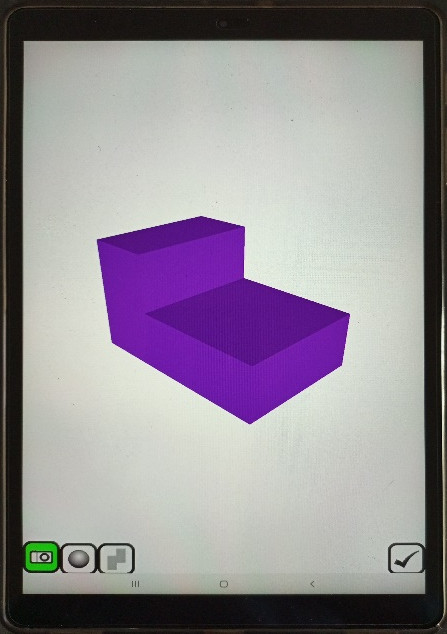
\includegraphics[width=\textwidth]{figures/figure01.jpg}
\caption{Interface do Qubism 3D Modeling.}
\label{fig-01}
\source{Elaboração própria.}
\end{minipage}
\end{figure}

\subsection{\emph{Software} de geometria dinâmica GeoGebra}\label{sub-sec-softwaredegeometriadinamica}

O software de geometria dinâmica GeoGebra, versão 5.0.721.0, é uma
ferramenta educacional livre, que permite potencializar a aprendizagem,
por meio da construção dos elementos geométricos, possibilitando a
percepção espacial da dinâmica da modelagem desses elementos. \textcite[p. 2]{alves2007} argumenta que \enquote{a utilização de softwares educativos nas
	aulas de geometria, especialmente os de geometria dinâmica, vem ao
	encontro dessas propostas, pois a utilização do computador ainda
	possibilita criar ambientes que fazem surgir novas formas de pensar e
	agir}. De acordo com o referido autor, as ferramentas do GeoGebra
permitem representar todos os conteúdos da geometria dinâmica, de modo a
impulsionar, de forma lógica, novas construções.

Particularmente para o estudo das SCs, o GeoGebra contém todos os
elementos para representar a seção produzida pelo plano secante,
permitindo esclarecer a transposição dos elementos geométricos em 3D
para 2D na folha de desenho. As ferramentas para a construção no
GeoGebra incluem ferramentas básicas de edição, pontos, transformações,
retas e polígonos (ver \Cref{fig-02}).

\begin{figure}[htpb]
\centering
\begin{minipage}{.4\textwidth}
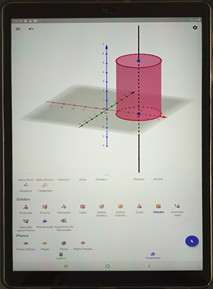
\includegraphics[width=\textwidth]{figures/figure02.jpg}
\caption{Interface do GeoGebra.}
\label{fig-02}
\source{Elaboração própria.}	
\end{minipage}
\end{figure}

\subsection{Visualização Espacial 3D}\label{sub-sec-Visualização Espacial 3D}

Visualização é o ato de observar um determinado foco, com o objetivo de
compreender todos os seus detalhes. Essa habilidade busca perceber um
objeto específico, sua composição ou ação. A Visualização Espacial é a
capacidade de observar mentalmente um determinado foco, para compreender
sua dinâmica. De acordo com \textcite[p. 2]{cohen2018},
\enquote{Consequently, these traditional psychometric spatial ability tests use
domain-general stimuli that bear little resemblance to authentic
engineering tasks} (Consequentemente, esses testes tradicionais de
habilidade espacial psicométrica usam estímulos de domínio geral, que
têm pouco em comum com tarefas de engenharia autênticas). Segundo \textcite[p. 224]{suzuki2002}, \enquote{a capacidade humana de reconhecer representações gráficas é chamada capacidade espacial ou capacidade de visualização espacial}.

Unindo os posicionamentos dos autores, VE é a habilidade de observar
espacialmente todos os detalhes do objeto, como cor, forma e posição.
Também pode ser considerada a habilidade de manipular mentalmente os
objetos no espaço para visualizar as vistas ortogonais. A capacidade
espacial nos conteúdos de Desenho Técnico e Geometria Descritiva permite
que o aluno visualize os objetos antes de resolver problemas em 2D na
folha de desenho. A habilidade espacial que se pretende que o aluno
tenha provém de um exercício mental, o que significa que, mesmo que o
aluno não tenha capacidade visioespacial, com um treinamento a partir de
exercícios progressivos e sistematizados, pode adquirir a habilidade de
VE. As disciplinas de DT e GD têm, portanto, como base, o
desenvolvimento da habilidade visual do aluno para resolver problemas de
representação e construções geométricas. Por isso, é necessária essa
habilidade para perceber mentalmente as formas e as relações dos
elementos geométricos espacialmente. Já as Projeções Ortogonais é um
tópico da disciplina de Desenho Técnico que estuda a representação de um
objeto em um plano de projeção. Uma projeção contém um conjunto de
elementos que, usando procedimentos específicos, são representados nos
planos correspondentes, permitindo diferentes vistas do objeto em
relação ao observador e proporcionando uma visão completa do mesmo
objeto através das vistas ortogonais. Por sua vez, a Seção de Cilindros
é a representação da seção produzida em um cilindro. Os elementos que
compõem a figura resultante da seção são determinados pela posição do
plano de corte.

\subsection{Mediação}\label{sub-sec-mediação}

A mediação pedagógica é um processo de interação dialógica, no qual
tanto professor quanto aluno aprendem e ensinam juntos, em construção,
pois quem ensina aprende ao ensinar e quem aprende ensina ao aprender
\cite{mori2013}. Podemos definir o processo de ensinar como uma sequência
de atividades do professor e dos alunos, visando a assimilação de
conhecimentos e o desenvolvimento de habilidades, por meio dos quais os
alunos aprimoram capacidades cognitivas, pensamento independente,
observação, análise-síntese e outras \cite[p. 54]{libaneo2013}. Por sua
vez, a aprendizagem caracteriza-se pela assimilação ativa de
conhecimentos e operações mentais, para compreendê-los e aplicá-los. É
uma forma do conhecimento humano - a relação cognitiva entre aluno e
matéria de estudo - desenvolvendo-se sob as condições específicas do
processo de ensino \cite{libaneo2013}. Na visão deste autor, a unidade
ensino-aprendizagem realiza-se na interligação de dois momentos
indissociáveis de transmissão e assimilação ativa de conhecimentos,
capacidades, em condições específicas de cada situação didática.

A mediação no ensino é o processo de aprendizagem e de interpretação dos
conteúdos planejados. Nesse processo, os intervenientes são o aluno, o
professor e a matéria. A mediação deve ser planejada com relevância para
uma prática educativa entre os intervenientes, em que o professor é o
principal agente, responsável por facilitar os conteúdos, e orientar a
construção do conhecimento no aluno, de forma colaborativa e com o
auxílio da tecnologia adequada aos conteúdos pretendidos. Vygotsky
distingue dois elementos básicos responsáveis pela mediação: o
instrumento, que tem a função de regular as ações sobre os objetos, e o
que regula as ações sobre o psiquismo das pessoas \cite[p. 50]{rego1995}.

A mediação didática deve facilitar o processo de aprendizagem e
proporcionar ao aluno uma assimilação que lhe permita construir os
conhecimentos. A realização didática tem como base a relação entre o
aluno e a matéria, com o objetivo de se apropriar dela com a mediação do
professor. O professor, nesse estágio, é um agente externo, servindo de
mediador entre o aluno e a matéria \cite{vygotskii1988}.





